
\documentclass[12pt,a4paper,titlepage,oneside]{article}
\usepackage[top=2.5cm, bottom=2cm, left=2.5cm, right=1cm]{geometry} 
% Font, accents
\usepackage[utf8]{inputenc}
\usepackage{fancyhdr}
\usepackage[T1]{fontenc}
\usepackage{times}     
% Interactive index
\usepackage{hyperref}
% Spanish titles
\usepackage[spanish]{babel}
% Attached files
\usepackage{attachfile}
\attachfilesetup{
  icon = Paperclip
}
% Fix curly verbatim apostrophes
\usepackage{upquote,textcomp}
% Make lists without bullets
\renewenvironment{itemize}{
 \begin{list}{}{
  \setlength{\leftmargin}{1.5em}
 }
}{
 \end{list}
}



%Customize things
\usepackage[margin=0pt,font=small,labelfont=bf]{caption}
\usepackage[pdftex]{graphicx}
\usepackage[usenames,dvipsnames]{xcolor}

% Sections and subsections colors
\usepackage{titlesec}
\titleformat{\section}
{\color{Blue}\normalfont\Large\bfseries}
{\color{Blue}\thesection}{1em}{}
\newcommand{\sectionbreak}{\clearpage}


% Document properties
\title{Facultad de Ingeniería\\Técnicas de Programación Concurrente I [75.59]}
\date{\today}
\hypersetup{
  colorlinks = true,
  urlcolor=blue,
  pdflang = es,
  pdfauthor = {Federico Farina},
  pdfproducer = {Federico Farina},
  pdfcreator = Texmaker,
  pdftitle = {TP1},
}

\begin{document}
   % code start
    \fancyhead[LE]{\leftmark} 
    \fancyhead[RO]{\rightmark} 
    \fancyhead[L]{Técnicas de Programación Concurrente I}
    \fancyhead[R]{TP1}    
    \renewcommand{\headrulewidth}{0.4pt} 
    \renewcommand{\footrulewidth}{0pt}
    % code end

    % set pagestyle to use fancy header and footer
    \pagestyle{fancy}


 \maketitle
  \setcounter{page}{1}
  \pagenumbering{roman}
  \tableofcontents

\newpage{}
\pagenumbering{arabic}
\setcounter{page}{1}

\section{Enunciado}

\subsection{Objetivo}

El objetivo de este proyecto consiste en implementar la simulación parcial del funcionamiento de una estación de servicio.

\subsection{Requerimientos Funcionales}

Esta simulacion abarcar a el funcionamiento de una estación de servicio. Los requerimientos funcionales son los siguientes:

\begin{enumerate}
\item 
La estacion de servicio cuenta con un número determinado de surtidores, un jefe de estación y un conjunto de empleados que atienden de a un auto por vez.
\item 
Tanto el número de surtidores disponibles como el número de empleados deben ser configurables y se establecen al inicio de la simulación.
\item
Cuando un auto llega a la estación de servicio es atendido en primer lugar por el jefe de estación quien asignará un empleado para atender al auto. Si no hay un empleado disponible, el auto se retira de la estación de servicio.
\item
El jefe de estación debe atender a los autos por orden de llegada de los mismos.
\item
Cuando el empleado recibe un auto de parte del jefe de estación, debe localizar un surtidor libre para atender al auto en cuestión. Si no encuentra ningú surtidor libre, deberá esperar hasta tanto se libere alguno.
\item
Una vez que el empleado obtiene un surtidor atiende al auto en cuestión. Mientras el empleado está atendiendo al auto no se puede utilizar el mismo surtidor para otro auto, ni el empleado es capaz de atender más de un auto a la vez.
\item
Finalmente, antes de que el auto se retire el empleado deberá cobrar el cargo correspondiente, el cual será almacenado en la caja de la estación de servicio.
\item
Todos los empleados guardan la recaudación en la misma caja y sólo un empleado puede utilizar la caja a la vez.
\item
Durante cualquier momento de la simulación, el administrador de la estación de servicio podrá consultar la recaudación guardada en la caja. Mientras lo hace, si algún empleado tiene recaudación para guardar, deberá esperar hasta que el administrador finalice su consulta.
\end{enumerate}

 
\subsection{Requerimientos no Funcionales}

Los siguientes son los requerimientos no funcionales de la aplicación:

\begin{enumerate}
 \item
  El proyecto deberá ser desarrollado en lenguaje C o C++, siendo este último el  lenguaje de preferencia.
  \item
  La simulación puede no tener interfaz gráfica y ejecutarse en una o varias consolas de línea decomandos.
  \item
  El proyecto deberá funcionar en ambiente Unix / Linux.
  \item
La aplicación deberá funcionar en una única computadora.  
\item
El programa deberá poder ejecutarse en "modo debug", lo cual dejará registro de la actividad que realiza en un único archivo de texto para su revisión posterior.
\end{enumerate} 


Las facilidades de IPC que se podrán utilizar para la realización de este proyecto son las que abarcan la primera parte de la materia, es decir, hasta el primer parcial. Dichas facilidades son: 
\begin{itemize}
\item[•] Memoria compartida
\item[•] Señales
\item[•] Pipes y fifos
\item[•] Locks
\item[•] Semaforos
\end{itemize}

Cualquier otra facilidad queda expresamente excluida para este proyecto.

\subsection{Tareas a Realizar}

A continuación se listan las tareas a realizar para completar el desarrollo del proyecto:

\begin{enumerate}
\item
 Dividir el proyecto en procesos. El objetivo es lograr que la simulación esté conformada por un conjunto de procesos que sean lo más sencillos posible.
\item
Una vez obtenida la división en procesos, establecer un esquema de comunicación entre ellos teniendo en cuenta los requerimientos de la aplicación. ¿Qué procesos se comunican entre sí?, ¿Qué datos necesitan compartir para poder trabajar?
\item
Tratar de mapear la comunicación entre los procesos a los problemas conocidos de concurrencia.
\item 
Determinar los mecanismos de concurrencia a utilizar para cada una de las comunicaciones entre procesos que fueron detectadas en el ítem 2. No se requiere la utilización de algún mecanismo específico, la elección en cada caso queda a cargo del grupo y debe estar debidamente justificada.
\item
 Realizar la codificación de la aplicación. El código fuente debe estar documentado.
\end{enumerate}
 
\subsection{Entrega} 

La entrega del proyecto comprende lo siguiente:

\begin{enumerate}
\item
Informe, se deberá presentar impreso en una carpeta o folio y en forma digital (PDF) a través del campus
\item
El código fuente de la aplicación, que se entregará únicamente mediante el campus
\end{enumerate}

La entrega en el campus estará habilitada hasta las 19 hs de la fecha indicada oportunamente.

El informe a entregar debe contener los siguientes ítems:

\begin{enumerate}
\item
Breve análisis del problema, incluyendo una especificación de los casos de uso de la aplicación.
\item
Detalle de resolución de la lista de tareas anterior.
\item
Diagrama que refleje los procesos, el flujo de comunicación entre ellos y los datos que intercambian.
\item
Diagramas de clases realizados.
\item
Diagrama de transición de estados del jefe de estación.
\end{enumerate}

\section{Objetivo}
El objetivo de este proyecto es el desarrollo de una aplicación conocida como ConcuStation.
Esta aplicación permitirá simular el funcionamiento de una estación de servicio. Al iniciar la aplicación, el usuario podrá decidir el número de empleados y surtidores que desee.
Los empleados atienden un auto por vez y almacenan la recaudación en una caja común. En todo momento se podrá consultar el saldo disponible en la caja.

\section{Análisis del problema}
Para el análisis del problema, se identificaron los actores que intervienen en el sistema. A continuación se presenta una breve descripción de cada uno.

\subsection{Actores}
\begin{enumerate}
\item[•] Jefe de estación: Encargado de recibir los autos que ingresan en la estación de servicio y asignar un empleado para su atención.
\item[•] Empleado: Encargado de atender los autos y almacenar la recaudación en la caja.
\item[•] Administrador: Consulta la recaudación disponible en la caja.
\end{enumerate}

\subsection{Casos de uso}
Se identificaron los siguientes casos de uso:

\begin{enumerate}
\item[•] Recibir auto
\item[•] Asignar empleado
\item[•] Atender auto
\item[•] Almacenar recaudación
\item[•] Consultar recaudación
\end{enumerate}

\begin{figure}[hbtp]
\centering
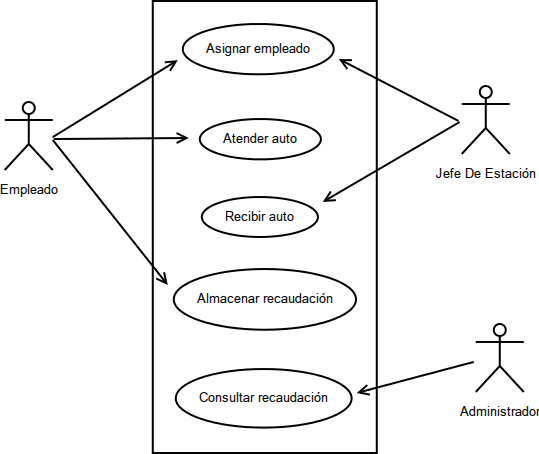
\includegraphics[scale=0.6]{diagramaDeCasosDeUso.png} 
\caption{Diagrama de Casos de Uso}
\end{figure}

\subsection{Caso de uso: Atender auto}
\begin{enumerate}
\item Descripción: El empleado atiende el auto asignado por el jefe de estación y almacena la recaudación en la caja.
\item Actores participantes: Empleado
\item Pre-condiciones: El auto a atender debe ser previamente asignado por el jefe de estación. Debe haber al menos un surtidor libre y el empleado no puede estar ocupado atendiendo otro auto. El tiempo de carga debe ser menor al tiempo de simulación restante.
\item Flujos
Flujo principal
Post condiciones: 
\end{enumerate}
\newpage

\section{Diagrama de estado}

A continuación mostramos el diagrama de estados correspondiente a las acciones del jefe de estación.
\bigskip

\begin{figure}[hbtp]
\centering
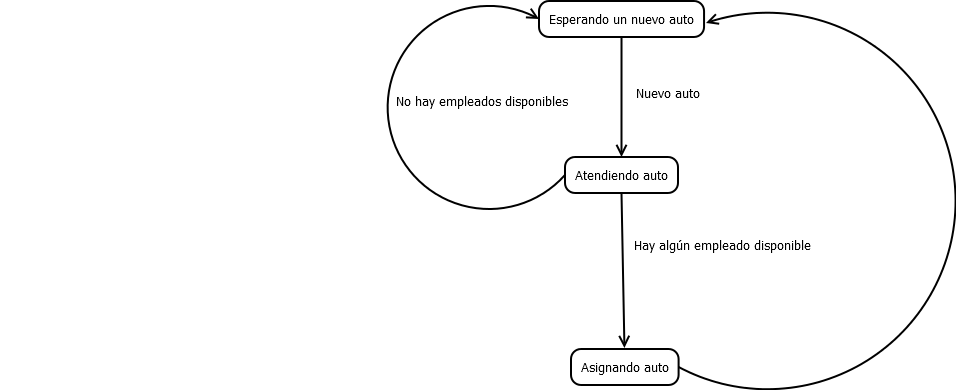
\includegraphics[scale=0.5]{diagrama_estado_jefe.png}
\caption[Long caption]{Diagrama de estado del jefe de estación}
\end{figure}


\section{Mapeo a problemas conocidos de concurrencia}

\bigskip


\begin{center}
   \begin{tabular}[1.5\textwidth]{| l | c |}
     \hline
     Dominio & Problema de Concurrencia  \\ \hline
     Entrada y atencion de autos & Productor-Consumidor  \\ \hline
     7 & 8  \\
     \hline
   \end{tabular}
 \end{center}
 
  

\section{Tareas realizadas}

\begin{enumerate}
\item Dividir el programa en procesos. El objetivo es lograr que cada programa participante este conformado por un conjunto de procesos que sean lo más sencillos posible.

\begin{itemize}
\item[•] Se crean dos procesos principales: Un proceso asociado a la vista (interfaz gráfica de usuario) y un proceso que controla el flujo de ejecución de la simulación.
\item[•] Se crea un proceso cada vez que entra un auto a la estación de servicio: Al ingresar es recibido por el jefe de estación, el cual busca algún empleado que se encuentre disponible para ser asignado a atender el auto. Si hay algún empleado disponible, se crea un nuevo proceso para atender el auto. La duración de la atención está determinada por la capacidad en litros del tanque de nafta del auto.
\end{itemize}

NOTA: Si la capacidad del auto que ingresa a la estación de servicio es mayor al tiempo de simulación disponible, no es posible atender el auto y el mismo se retira de la estación de servicio; al igual que en el caso de no haber empleados disponibles.

\item Una vez obtenida la división en procesos, establecer un esquema de comunicación entre ellos teniendo en cuenta los requerimientos de la aplicación. ¿Qué procesos se comunican entre sí? ¿Qué datos necesitan compartir para poder trabajar?

\begin{itemize}
\item[•] El proceso principal se comunica con la vista por medio de un canal de comunicación. Al ingresar un nuevo auto, se puede determinar su capacidad mediante la interfaz gráfica de usuario. La vista escribe en el canal dicha capacidad y el proceso principal la lee para determinar el tiempo que necesita el auto en ser atendido.
\item[•] El proceso principal y los procesos responsables de atender los autos que ingresan en la estación de servicio dejan el registro de su actividad en un único archivo de texto si el programa es ejecutado en modo debug. Este archivo debe ser compartido por todos los procesos.
\item[•] Cada vez que se lanza un proceso para atender un nuevo auto, el proceso escribe la recaudación resultante en una caja común. Esta caja es compartida por todos los procesos y por el administrador de la estación de servicio, el cual en todo momento puede consultar la recaudación contenida en la caja.
\item[•] La vista debe comunicar al proceso principal la finalización del tiempo de simulación. Este tiempo es controlado por la vista mediante un timer.
\end{itemize}

\item Tratar de mapear la comunicación entre los procesos a los problemas conocidos de concurrencia.

\item Determinar los mecanismos de concurrencia a utilizar para cada una de las comunicaciones entre procesos que fueron detectadas en el ítem 2. No se requiere la utilización de algún mecanismo específico, la elección en cada caso queda a cargo del grupo y debe estar debidamente justificada.

\begin{itemize}
\item[•] Si el programa es ejecutado en modo debug, se utiliza un Lock File para sincronizar correctamente la escritura de los procesos en el archivo de texto.
\item[•] Para determinar la cantidad de surtidores libres, se utiliza un semáforo inicializado en la cantidad de surtidores disponibles. Cada vez que ingresa un nuevo auto, el proceso lanzado intenta entrar en el semáforo, lo cual decrementa el valor del mismo. Si no hay surtidores libres, es decir, si el valor del semáforo es igual a 0, el proceso queda en espera hasta tanto algún otro proceso libere el semáforo incrementando su valor. Esta situación ocurre cuando ingresa un nuevo auto y el empleado asignado para su atención no encuentra un surtidor libre.
\item[•] La caja es una memoria compartida por todos los procesos que se lanzan cada vez que ingresa un nuevo auto. Dado que estos procesos pueden ejecutarse concurrentemente, se utiliza un semáforo de exclusión mutua para la sincronización de la lectura y escritura en la memoria compartida.
\end{itemize}
\end{enumerate}

\section{Diagrama de Clases}
\begin{figure}[hbtp]
\centering
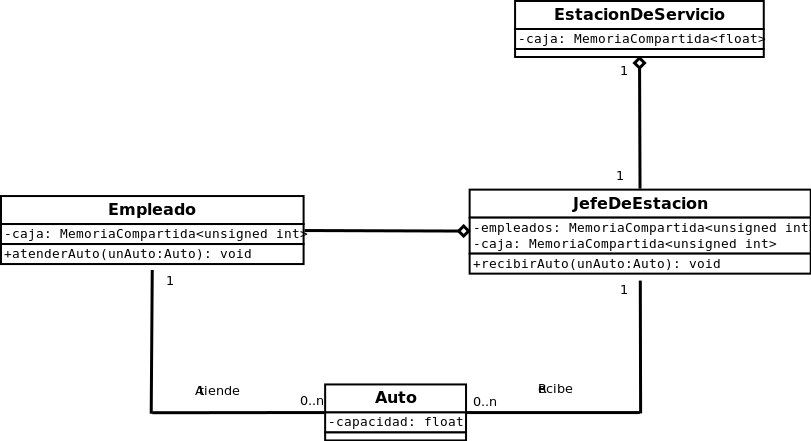
\includegraphics[scale=0.5]{diagramaDeClases.png}
\caption{Diagrama de Clases}
\end{figure}

\end{document}